\documentclass[11pt,letterpaper]{article}
\usepackage{fullpage}
\usepackage[top=2cm, bottom=2cm, left=1cm, right=1cm]{geometry}
\usepackage{fancyhdr}
\usepackage{enumitem}
\usepackage{graphicx}
\usepackage{wrapfig}
% Feel free to add packages!

% First page setup (do not edit)
\fancypagestyle{firstpagestyle}
{
\headheight 35pt
\lhead{\nameA}
\lhead{\nameA\\\nameB}                 
\chead{\textbf{\large Questions Group \groupnumber}}
\rhead{\nameC \\\nameD }
\headsep 1.5em
\topmargin = -54pt
}

% Please fill in all unknows here
\newcommand\groupnumber{GRPNR}          % <-- group number #HERE
\newcommand\nameA{Giuseppe Gianfraneschi}               % <-- Names #HERE
\newcommand\nameB{name B}               % <-- Names #HERE
\newcommand\nameC{name C}               % <-- Names #HERE
\newcommand\nameD{name D}               % <-- Names #HERE


\begin{document}
\thispagestyle{firstpagestyle}\noindent

\begin{enumerate}[leftmargin=5mm,topsep=0pt,itemsep=0ex,partopsep=1ex,parsep=1ex]
	\item Your answers to Question 1 go here. In all answers, please adhere to the instructions in \texttt{organization.pdf}. Keep in mind the one-page limit (excluding potential references) and don't forget to fill in your names and group number.
	\item {One way to detect overfitting is to compare model performance against a validation data set. By varying, for example, tree depth when fitting a random forest classifier, performance gain can be compared in both data sets against depth of the model. As decision trees often suffer from overfitting when model depth is large, the optimal tree depth can be determined this way.
	As can be seen in Fig \ref{fig:score-tree-depth}, the validation score stabilises only after increasing the tree depth to about 20. At this level the training data already gives a score of almost 1.0. This means that not overfitting of the training data is happening as increasing the tree depth does not further increase the training score, while also not further decreasing the validation score
	}
	\item Your answers to Question 3 go here.
	\item Your answers to Question 4 go here.
	\item Your answers to Question 5 go here.
	\item Your answers to Question 6 go here.
\end{enumerate}
\newpage
\section*{Appendix}
\begin{figure}[!ht]
	\centering
	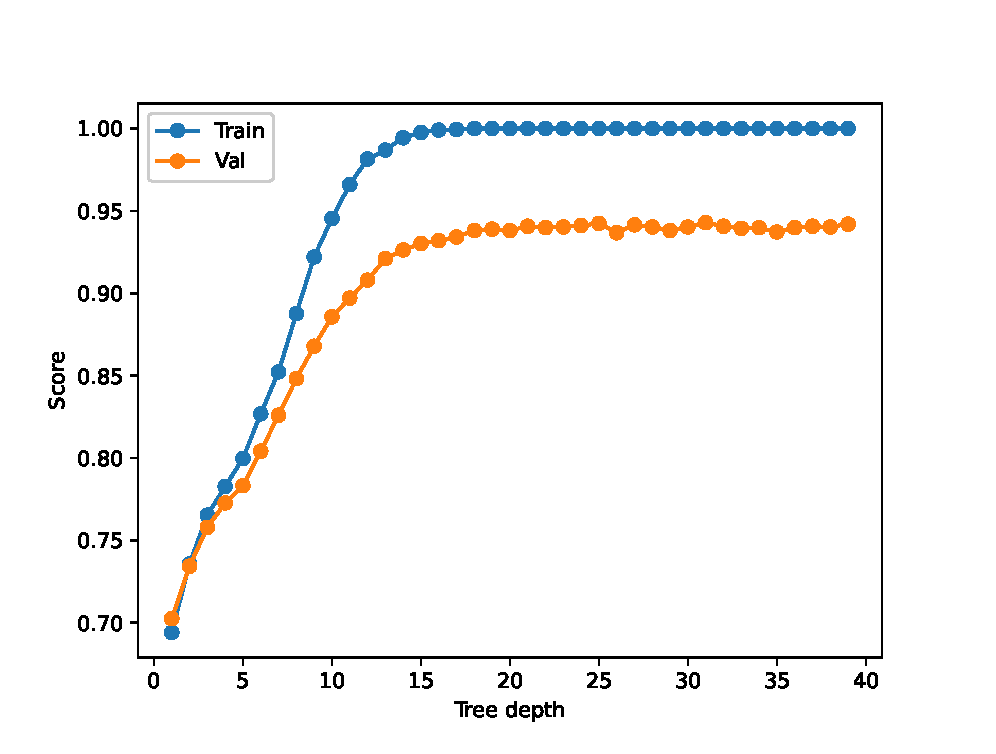
\includegraphics[width=0.7\textwidth]{img/overfit_plot.eps}
	\caption{Score vs Tree-depth}
	\label{fig:score-tree-depth}
\end{figure}

\newpage

\section*{References}
Your references go here. Feel free to use any packages you need to streamline your referencing. 

\end{document}



